\documentclass{beamer}
\usetheme{PaloAlto}
%\usecolortheme{crane}

\addtobeamertemplate{footline}
{%
   \usebeamercolor[fg]{author in sidebar}
   \vskip-1cm\hskip10pt
   %\insertpagenumber\,/\,\insertpresentationendpage\kern1em\vskip2pt%
   \insertframenumber\,/\,\inserttotalframenumber\kern1em\vskip2pt%
}

\usepackage{tikz}
\usepackage{booktabs}

\usetikzlibrary{arrows}
\usetikzlibrary{shapes}
\usetikzlibrary{patterns}
\usetikzlibrary{intersections}
\usetikzlibrary{calc}
\usetikzlibrary{fadings}

\tikzstyle{IpNode}=[rectangle, draw=black, thick, inner sep=12pt]
\tikzstyle{NewIpNode}=[IpNode, fill=green]
\tikzstyle{MacNode}=[circle, draw=black, thick, inner sep=7pt]
\tikzstyle{NewMacNode}=[MacNode, fill=green]

\tikzstyle{OpenEdge}=[->, ultra thick]
\tikzstyle{CloseEdge}=[OpenEdge, red]
\tikzstyle{VirtualEdge}=[CloseEdge, double]
\tikzstyle{NewOpenEdge}=[OpenEdge, densely dashed]
\tikzstyle{NewCloseEdge}=[CloseEdge, densely dashed]
\tikzstyle{NewVirtualEdge}=[VirtualEdge, densely dashed]

\tikzstyle{Input}=[shape=document, draw=black, fill=cyan, fill opacity=0.2, text opacity=1, thick, align=center, minimum width=15mm, minimum height=20mm]
\tikzstyle{Module}=[rectangle, draw=black, fill=blue, fill opacity=0.2, text opacity=1, thick, inner sep=10pt, align=center]
\tikzstyle{Library}=[rounded corners, draw=black, fill=green, fill opacity=0.2, text opacity=1, thick, inner sep=7pt, align=center]
\tikzstyle{Output}=[shape=document, draw=black, fill=violet, fill opacity=0.4, text opacity=1, thick, inner sep=7pt, align=center, minimum width=15mm, minimum height=20mm]
\tikzstyle{connection}=[-latex, line width=0.7mm, draw=black]
\tikzstyle{double connection}=[latex-latex, line width=0.7mm, draw=black]



\title[Reconstrucción y detección de tráfico]{Reconstrucción de caminos y detección de dispositivos}
\institute{Tutor: Guillermo Julián Moreno\\Ponente: Javier Aracil Rico\\\vskip 0.3cmUniversidad Autónoma de Madrid\\
    Ingeniería Informática y Matemáticas}
\author{David Moreno Maldonado}
\date{15 junio, 2020}

\begin{document}

\begin{frame}
\titlepage
\end{frame}

\begin{frame}
    \tableofcontents
\end{frame}

\section{Introducción}
\fontsize{10}{5}\selectfont
\begin{frame}{Descripción general}
\textbf{Situación:}
\begin{itemize}
    \item Existencia de redes de gran tamaño y complejidad.
    \item Varios puntos de captura de tráfico en estas redes.
\end{itemize}
\vskip 0.2cm

\textbf{Problemas:}
\begin{columns}
    \begin{column}{0.42\textwidth}
    \begin{itemize}
        \item Pérdida de paquetes.
        \item Ralentización de red.
        \item Paquetes duplicados.
    \end{itemize}
    \end{column}
    
    \begin{column}{0.08\textwidth}
        \vskip 0.1cm
        $\implies$
    \end{column}

    \begin{column}{0.45\textwidth}
    \vskip 0.1cm
    Necesidad de \textbf{detectar los puntos exactos} de la red donde se producen estos problemas.
    \end{column}
\end{columns}
\vskip 0.2cm

\textbf{Solución:}
\begin{center}
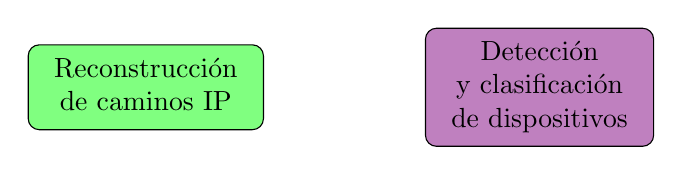
\begin{tikzpicture}
    \node (rec) [rectangle, rounded corners, centered, draw=black, fill=green!50] at (0,0){\begin{tabular}{c}
         Reconstrucción\\ de caminos IP
    \end{tabular}};
    \node (det) [rectangle, rounded corners, centered, draw=black, fill=violet!50] at (5,0) {\begin{tabular}{c}
         Detección\\y clasificación\\ de dispositivos
    \end{tabular}};
\end{tikzpicture}
\end{center}

\textbf{Objetivos:}
\begin{itemize}
    \item Eficiencia en tiempo de ejecución y uso de memoria.
    \item Abstracción para su uso en diferentes entornos.
\end{itemize}
\end{frame}

\section{Estado del arte}
\begin{frame}{Reconstrucción de flujos IP}
\begin{itemize}
    \item Trazas \textit{pcap} capturadas.
    \item Útiles como herramientas auxiliares.
    \item Análisis no específico en reconstrucción.
    \item Poca eficiencia con trazas de gran tamaño.
\end{itemize}
\vskip 0.7cm
\begin{columns}
    \begin{column}{0.3\textwidth}
        \centering
        
\includegraphics[scale=0.05]{img/wireshark.png}
    \end{column}
    \begin{column}{0.3\textwidth}
        
\includegraphics[scale=0.2]{img/netflow.png}
    \end{column}
    \begin{column}{0.3\textwidth}
        
\includegraphics[scale=0.6]{img/capsa.png}
    \end{column}
\end{columns}
    
\end{frame}

\begin{frame}{Detección de dispositivos}
\begin{itemize}
    \item No existen métodos generalizados.
    \item Estudio de las características para inferir el dispositivo.
    \item Existencia de dispositivos compuestos.
\end{itemize}
\vskip 0.7cm
\begin{columns}
    \begin{column}{0.3\textwidth}
        \centering
        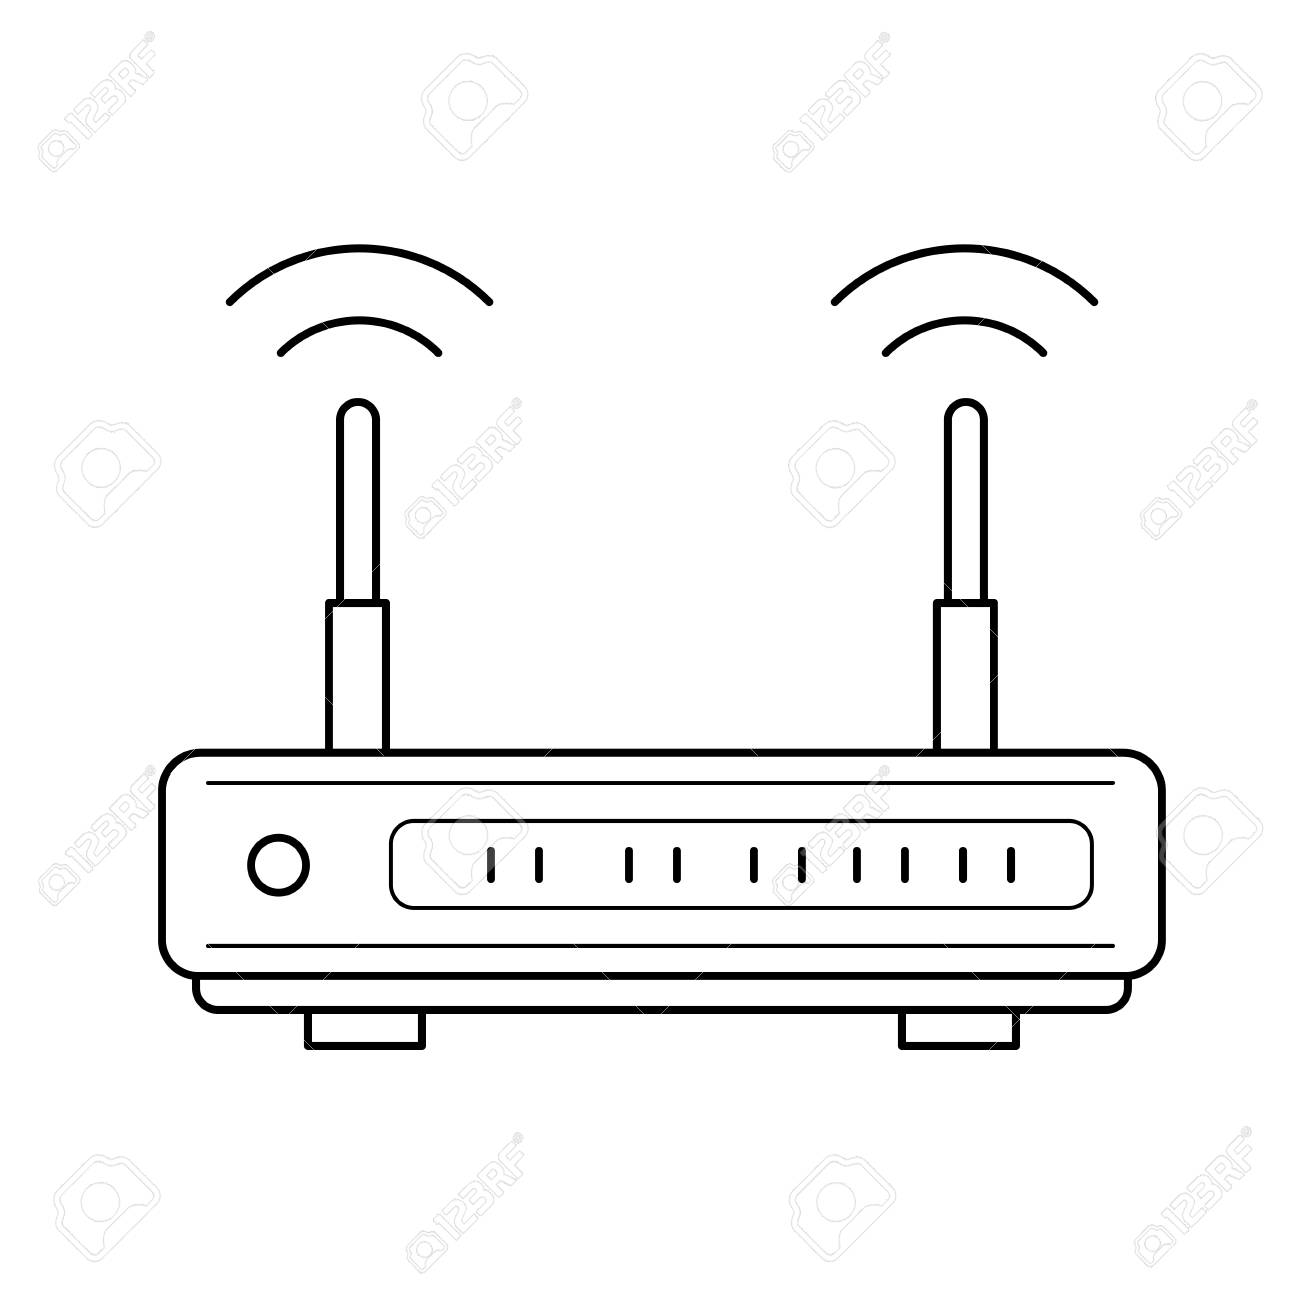
\includegraphics[scale=0.2]{img/router.jpg}
    \end{column}
    \begin{column}{0.3\textwidth}
        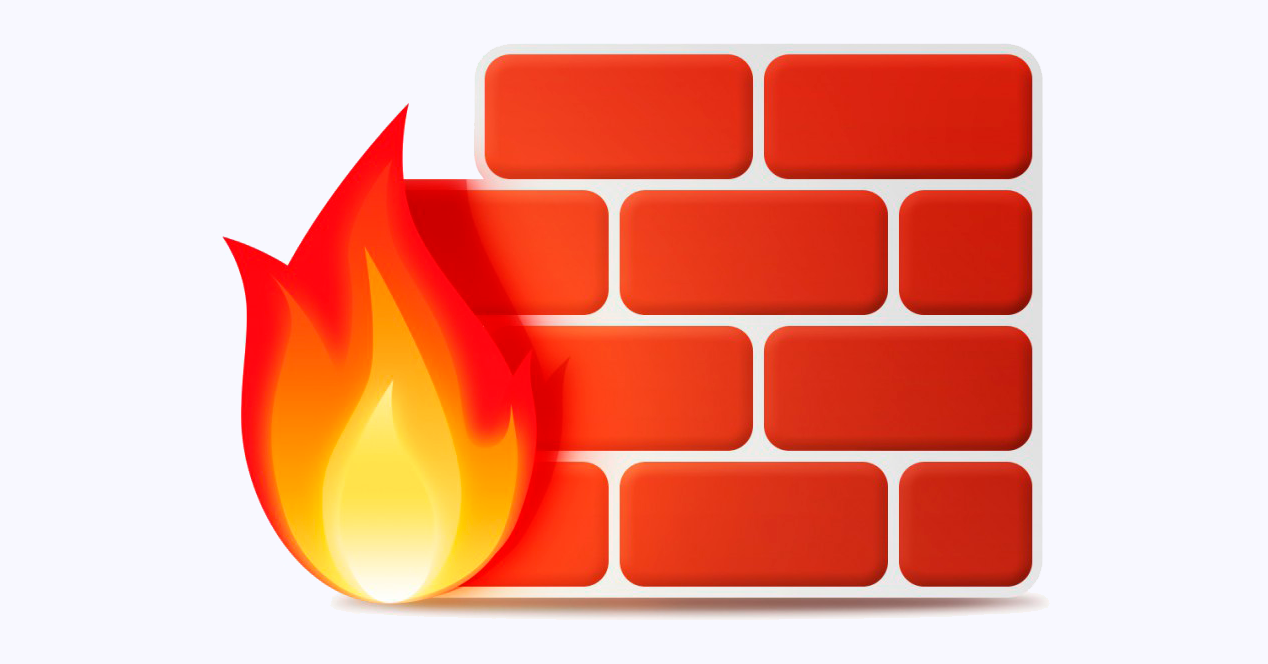
\includegraphics[scale=0.1]{img/firewall.png}
    \end{column}
    \begin{column}{0.3\textwidth}
        
\includegraphics[scale=0.3]{img/load_balancer.png}
    \end{column}
\end{columns}
    
\end{frame}

\section{Análisis del problema}
\subsection{Reconstrucción de caminos}
\begin{frame}{Planteamiento del problema y caso inicial}
\begin{itemize}
    \item La información recibida es a nivel de paquete con IP origen y destino y MAC origen y destino.
    \item Almacenar los flujos IP en un grafo unidireccional.
    \item Aristas abiertas y cerradas dependiendo de si la conexión entre nodos se ha visto físicamente.
\end{itemize}
\begin{figure}
    \scalebox{.7}{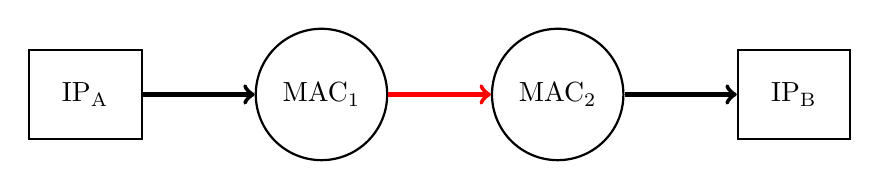
\begin{tikzpicture}
\node[IpNode](IPA) at (0,0) {IP\textsubscript{A}};
\node[MacNode](MAC1) at (3,0) {MAC\textsubscript{1}};
\node[MacNode](MAC2) at (6,0) {MAC\textsubscript{2}};
\node[IpNode](IPB) at (9,0) {IP\textsubscript{B}};

\draw[OpenEdge](IPA) -- (MAC1);
\draw[CloseEdge](MAC1) -- (MAC2);
\draw[OpenEdge](MAC2) -- (IPB);

\end{tikzpicture}}
\end{figure}
\end{frame}

\begin{frame}{Inserción estándar}
Cuando vemos un paquete con MAC destino igual al primer nodo MAC del grafo:
\begin{figure}
    \scalebox{.7}{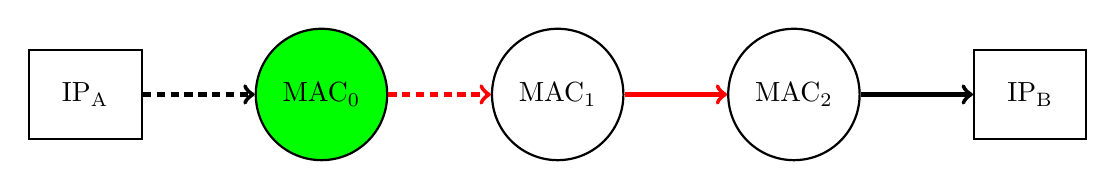
\begin{tikzpicture}
\node[IpNode](IPA) at (0,0) {IP\textsubscript{A}};
\node[NewMacNode](MAC0) at (3,0) {MAC\textsubscript{0}};
\node[MacNode](MAC1) at (6,0) {MAC\textsubscript{1}};
\node[MacNode](MAC2) at (9,0) {MAC\textsubscript{2}};
\node[IpNode](IPB) at (12,0) {IP\textsubscript{B}};

\draw[NewOpenEdge](IPA) -- (MAC0);
\draw[NewCloseEdge](MAC0) -- (MAC1);
\draw[CloseEdge](MAC1) -- (MAC2);
\draw[OpenEdge](MAC2) -- (IPB);
\end{tikzpicture}}
\end{figure}
\vskip 0.3cm
Cuando vemos un paquete con MAC origen igual al último nodo MAC del grafo:
\begin{figure}
    \scalebox{.7}{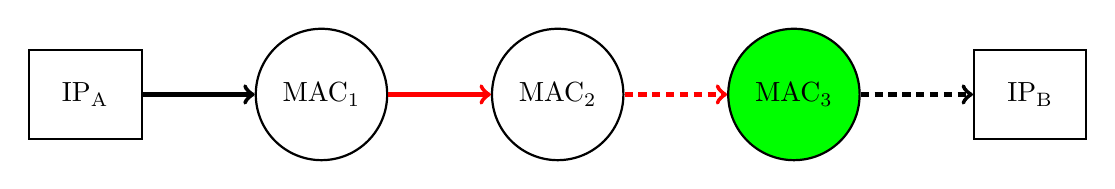
\begin{tikzpicture}
\node[IpNode](IPA) at (0,0) {IP\textsubscript{A}};
\node[MacNode](MAC1) at (3,0) {MAC\textsubscript{1}};
\node[MacNode](MAC2) at (6,0) {MAC\textsubscript{2}};
\node[NewMacNode](MAC3) at (9,0) {MAC\textsubscript{3}};
\node[IpNode](IPB) at (12,0) {IP\textsubscript{B}};

\draw[OpenEdge](IPA) -- (MAC1);
\draw[CloseEdge](MAC1) -- (MAC2);
\draw[NewCloseEdge](MAC2) -- (MAC3);
\draw[NewOpenEdge](MAC3) -- (IPB);
\end{tikzpicture}}
\end{figure}
\end{frame}

\begin{frame}{Bifurcación}
¿Por qué ocurren?
\begin{itemize}
    \item Caída temporal de una parte de la red.
    \item Congestión de la red.
    \item Funcionamiento usual de la red.
\end{itemize}
\vskip 0.2cm
Las detectamos cuando observamos un paquete con un nodo MAC en el grafo, pero no estamos en el caso de inserción estándar:
\begin{figure}
    \scalebox{.7}{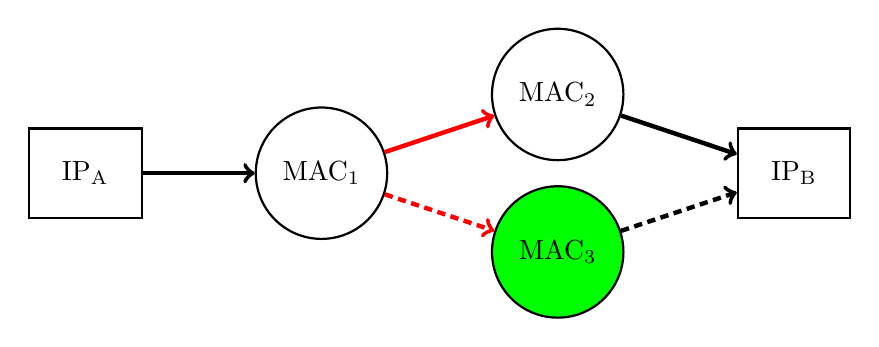
\begin{tikzpicture}
\node[IpNode](IPA) at (0,1) {IP\textsubscript{A}};
\node[MacNode](MAC1) at (3,1) {MAC\textsubscript{1}};
\node[MacNode](MAC2) at (6,2) {MAC\textsubscript{2}};
\node[NewMacNode](MAC3) at (6,0) {MAC\textsubscript{3}};
\node[IpNode](IPB) at (9,1) {IP\textsubscript{B}};

\draw[OpenEdge](IPA) -- (MAC1);
\draw[CloseEdge](MAC1) -- (MAC2);
\draw[NewCloseEdge](MAC1) -- (MAC3);
\draw[NewOpenEdge](MAC3) -- (IPB);
\draw[OpenEdge](MAC2) -- (IPB);
\end{tikzpicture}}
\end{figure}
\end{frame}

\begin{frame}{Camino huérfano}
\begin{array}{ccc}
    \mbox{Analizamos un paquete} & & \mbox{Necesitamos utilizar}\\
    \mbox{cuyas MAC no están} & \implies & \mbox{información extra.}\\
    \mbox{en el grafo.} & & \mbox{TTL del paquete.}
\end{array}
\vskip 0.4cm
Se genera una arista virtual conectando los nodos.
\begin{figure}
    \scalebox{.7}{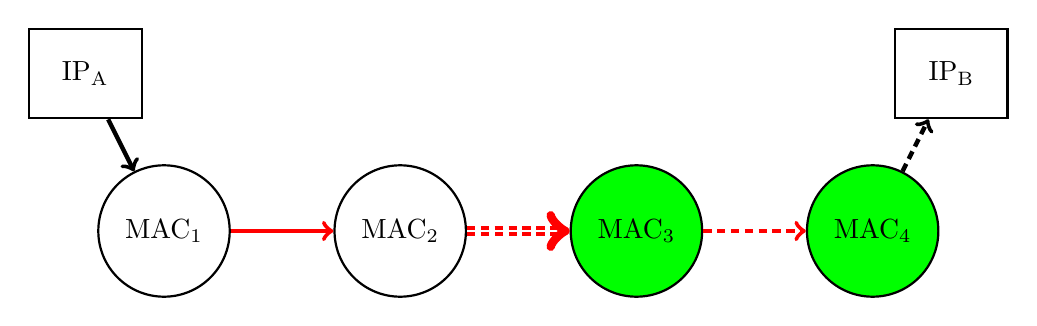
\begin{tikzpicture}
\node[IpNode](IPA) at (0,0) {IP\textsubscript{A}};
\node[MacNode](MAC1) at (1,-2) {MAC\textsubscript{1}};
\node[MacNode](MAC2) at (4,-2) {MAC\textsubscript{2}};
\node[NewMacNode](MAC3) at (7,-2) {MAC\textsubscript{3}};
\node[NewMacNode](MAC4) at (10,-2) {MAC\textsubscript{4}};
\node[IpNode](IPB) at (11,0) {IP\textsubscript{B}};

\draw[OpenEdge](IPA) -- (MAC1);
\draw[CloseEdge](MAC1) -- (MAC2);
\draw[NewVirtualEdge](MAC2) -- (MAC3);
\draw[NewCloseEdge](MAC3) -- (MAC4);
\draw[NewOpenEdge](MAC4) -- (IPB);
\end{tikzpicture}}
\end{figure}
%Problemas con el orden de los paquetes en las trazas \textit{pcap} en relación a los \textit{firewalls}.
\end{frame}

\subsection{Identificación y clasificación de dispositivos}
\begin{frame}{Identificación de dispositivos}
\begin{enumerate}
    \item Identificamos como dispositivos las aristas virtuales.
    \item Agregamos la información de todos los flujos (MAC de entrada y de salida, bytes, \textit{frames}, ...).
    \item Resolvemos las dependencias existentes entre dispositivos.
\end{enumerate}
%TODO: FLowchart con el algoritmo
    
\end{frame}

\begin{frame}{Clasificación de los dispositivos}
Diferenciamos entre \textit{firewalls}, \textit{routers} y balanceadores de carga a nivel MAC. Se siguen estas reglas:
\begin{enumerate}
    \item Los dispositivos con $\Delta \mbox{TTL} = 0$ se clasifican como \textit{firewalls}.
    \item Aquellos que conecten más de una MAC física y \textit{unicast} se clasifican como balanceadores de carga a nivel MAC.
    \item El resto se clasifica como \textit{router}.
\end{enumerate}
\end{frame}

\section{Desarrollo}
\subsection{Decisiones generales}
\begin{frame}{Planteamiento inicial del desarrollo}
El programa se desarrollo para la empresa Naudit, dedicada al análisis y monitorización de redes.
\vskip 0.5cm
\begin{array}{ccccc}
    \mbox{Intento de} & & \mbox{Poca} & & \mbox{Utilizamos} \\
    \mbox{herramienta similar} & \implies & \mbox{eficiencia} & \implies & \mbox{C para el}\\
    \mbox{en Python} & & \mbox{en tiempo} & & \mbox{desarrollo}
\end{array}

\end{frame}

\begin{frame}{Integración con \textit{fisher}}
\begin{itemize}
    \item Aplicación dedicada a la lectura de trazas pcap. 
    \item Se utilizaron y modificaron librerías internas (estructuras IP y MAC, diccionarios, listas, log, test).
    \item Uso de memoria estática. Se evita el uso continuo de \texttt{malloc} y \texttt{free}.
\end{itemize}
\end{frame}

\subsection{Estructura del programa}
\begin{frame}{Estructura general del programa}
    \begin{figure}
    \scalebox{.55}{\makeatletter
\pgfdeclareshape{document}{
\inheritsavedanchors[from=rectangle] % this is nearly a rectangle
\inheritanchorborder[from=rectangle]
\inheritanchor[from=rectangle]{center}
\inheritanchor[from=rectangle]{north}
\inheritanchor[from=rectangle]{south}
\inheritanchor[from=rectangle]{west}
\inheritanchor[from=rectangle]{east}
% ... and possibly more
\backgroundpath{% this is new
% store lower right in xa/ya and upper right in xb/yb
\southwest \pgf@xa=\pgf@x \pgf@ya=\pgf@y
\northeast \pgf@xb=\pgf@x \pgf@yb=\pgf@y
% compute corner of ‘‘flipped page’’
\pgf@xc=\pgf@xb \advance\pgf@xc by-10pt % this should be a parameter
\pgf@yc=\pgf@yb \advance\pgf@yc by-10pt
% construct main path
\pgfpathmoveto{\pgfpoint{\pgf@xa}{\pgf@ya}}
\pgfpathlineto{\pgfpoint{\pgf@xa}{\pgf@yb}}
\pgfpathlineto{\pgfpoint{\pgf@xc}{\pgf@yb}}
\pgfpathlineto{\pgfpoint{\pgf@xb}{\pgf@yc}}
\pgfpathlineto{\pgfpoint{\pgf@xb}{\pgf@ya}}
\pgfpathclose
% add little corner
\pgfpathmoveto{\pgfpoint{\pgf@xc}{\pgf@yb}}
\pgfpathlineto{\pgfpoint{\pgf@xc}{\pgf@yc}}
\pgfpathlineto{\pgfpoint{\pgf@xb}{\pgf@yc}}
\pgfpathlineto{\pgfpoint{\pgf@xc}{\pgf@yc}}
}
}
\makeatother

\begin{tikzpicture}
\begin{scope}
\fill[dashed, vlepsbasedseven, opacity=.5, draw opacity=1,  draw=black, ultra thick] (1.5, 2) rectangle (11, -6.5);

\node[Input](pcap) at (0,0) {Traza\\ pcap};
\node[Input](procesa) at (0,-3) {Fichero\\ \textit{Procesa}};
\node[Module](sfpcap) at (3.2,0) {Módulo\\ PCAP};
\node[Module](sfprocesa) at (3.2,-3) {Módulo\\ \textit{Procesa}};
\node[Module](sfipmac) at (7.5,-1.5) {Módulo\\ IPMAC};
\node[Library](layerlist) at (6, -5) {Librería\\ ordenación\\ superflujos};
\node[Library](devicesdetection) at (9, -5) {Librería\\ detección\\ dispositivos};
\node[Output](superflows) at (13, 0) {Salida\\superflujos\\ (registros)};
\node[Output](devices) at (13, -3) {Salida\\ dispositivos\\ (json)};

\draw[->, connection] (pcap.east) -- (sfpcap.west);
\draw[connection] (procesa.east) -- (sfprocesa.west);
\draw[connection] (sfpcap.east) -- (sfipmac.west);
\draw[connection] (sfprocesa.east) -- (sfipmac.west);
\draw[connection] (sfipmac.east) -- (superflows.west);
\draw[connection] (sfipmac.east) -- (devices.west);
\draw[double connection] (sfipmac.south) -- (layerlist.north);
\draw[double connection] (sfipmac.south) -- (devicesdetection.north);

\end{scope}

\end{tikzpicture}}
    \end{figure}
\end{frame}

\begin{frame}{Librería de ordenación de superflujos}
Librería abstracta, capaz de manejar flujos multicapa de diferentes características.
Estructuras de datos definidas:
\begin{itemize}
    \item Grafo unidireccional.
    \item Información de cada capa.
    \item Nodos.
    \item Aristas.
    \item Camino: Enlace entre estructuras externas.
\end{itemize}

Es necesario indicar la memoria disponible para estos elementos.
\end{frame}

\begin{frame}{Módulo IP/MAC}
\begin{itemize}
    \item Especifica la librería de ordenación de flujos para las capas IP y MAC
    \item Encargada de definir el número de estructuras de cada tipo requerido.
\end{itemize}

\begin{table}
	\begin{tabular}{lcc}
		\toprule \textbf{Estructura} & \textbf{Número de estructuras} \\ 
		& \textbf{por superflujo}\\
		\midrule
		Superflujos & 1 \\
		Elementos IP & 2 \\
		Elementos MAC & $\alpha$ \\
		Nodos & $2 + \alpha$ \\
		Aristas & $(\mbox{nodos} - 1) + \lambda$  \\ \bottomrule
	\end{tabular}
\end{table}
    
\end{frame}

\begin{frame}{Entrada al programa}

Ficheros \textit{pcap}:
\begin{itemize}
    \item Aprovecha totalmente la estructura interna de \textit{fisher}.
    \item Formato estándar de captura de tráfico.
\end{itemize}

Ficheros \textit{Procesa}:
\begin{itemize}
    \item Fichero por registros de conexiones. Formato interno Naudit.
    \item Ficheros más compactos que los \textit{pcap}.
    \item Necesidad de calcular menos datos internamente (RTT, número de \textit{frames}, ...).
\end{itemize}
    
\end{frame}

\begin{frame}{Salida del programa}

Salida de los superflujos:
\begin{itemize}
    \item Un registro por arista en el grafo
    \item Se indica información recopilada (número de \textit{frames}, bytes, ...)
\end{itemize}

Salida de dispositivos:
\begin{itemize}
    \item Formato JSON
    \item Información sobre interfaces MAC del dispositivo, flujo de paquetes y bytes o IPs que conecta.
\end{itemize}
    
\end{frame}

\section{Tests y resultados}
\subsection{Pruebas de código}
\begin{frame}{Pruebas realizadas al programa}
\begin{itemize}
    \item Uso del módulo de test integrado en \textit{fisher}.
    \item Test específicos para las librerías de ordenación y clasificación.
    \item Uso del CI (\textit{Continuous Integration}) disponible en GitLab.
    \item Depuración de memoria usada con Valgrind.
\end{itemize}
    
\end{frame}

\subsection{Resultados con trazas reales}
\begin{frame}{Tiempo de ejecución}
\centering
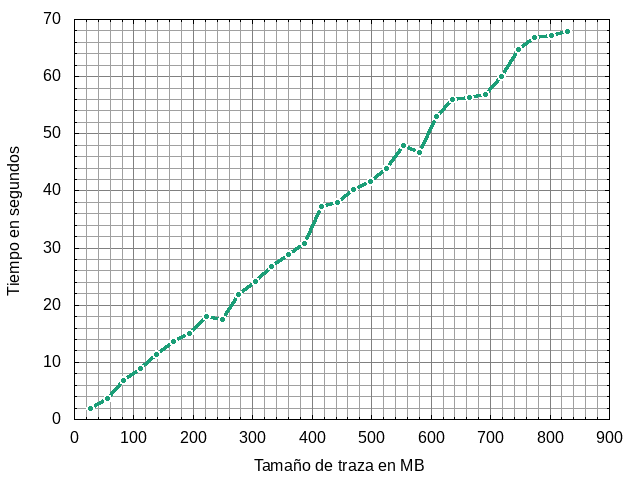
\includegraphics[scale=0.5]{gnuplot/png/time_ordering.png}
\end{frame}

\begin{frame}{Uso de memoria}
\centering
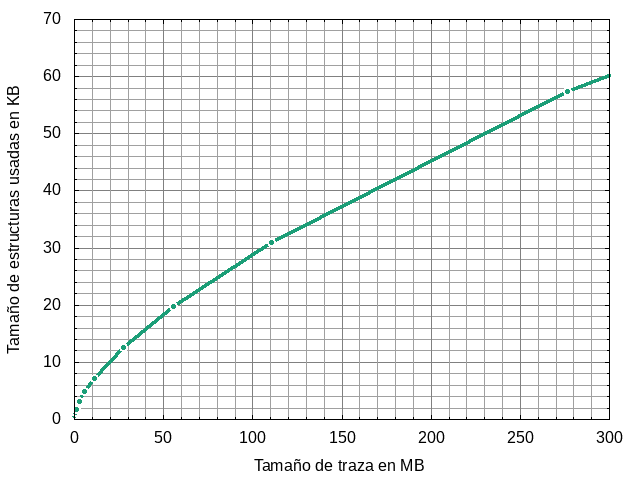
\includegraphics[scale=0.5]{gnuplot/png/memory-usage.png}
    
\end{frame}

\section{Trabajo futuro}
\begin{frame}{Trabajo futuro}
\begin{itemize}
    \item Aumento de la información recopilada en cada dispositivo, por ejemplo, subredes.
    \item Clasificación más detallada (balanceadores de carga a nivel IP, routers NAT, ...).
\end{itemize}
    
\end{frame}

\begin{frame}{}
  \centering \huge
  \emph{Muchas gracias.}
\end{frame}

\end{document}